\documentclass[tikz,border=8pt]{standalone}
\usepackage{amsmath}
\usepackage{amssymb}
\usepackage{tikz}
\usetikzlibrary{arrows.meta,calc,decorations.pathreplacing,patterns,shapes.geometric,positioning,shadings,plotmarks}

\begin{document}
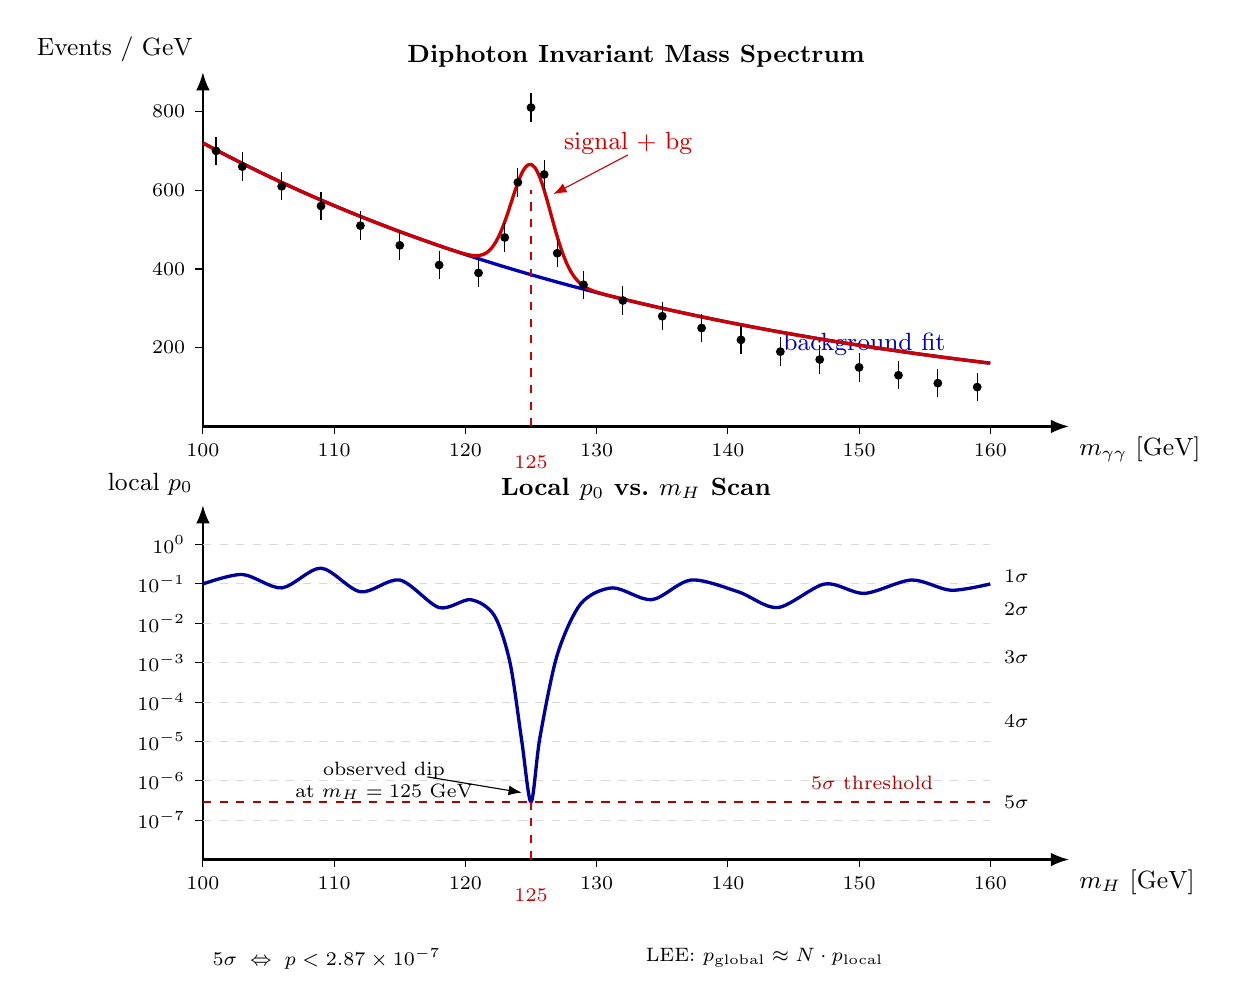
\begin{tikzpicture}[>=Latex]

%==================== TOP PANEL: m_gamma_gamma spectrum ====================
\begin{scope}[shift={(0,5.5)}]

% Axes
\draw[->, thick] (0,0) -- (11,0) node[below right] {\small $m_{\gamma\gamma}$ [GeV]};
\draw[->, thick] (0,0) -- (0,4.5) node[above left] {\small Events / GeV};

% x-axis ticks
\foreach \m in {100,110,120,130,140,150,160}{
  \pgfmathsetmacro{\xc}{(\m-100)/6}
  \draw (\xc,0) -- (\xc,-0.1) node[below] {\scriptsize \m};
}

% y-axis ticks
\foreach \y/\lab in {1/200,2/400,3/600,4/800}{
  \draw (0,\y) -- (-0.1,\y) node[left] {\scriptsize \lab};
}

% Background curve: smooth decreasing exponential-like polynomial
\draw[blue!70!black, very thick, smooth, samples=80, domain=0:10]
  plot (\x,{3.6*exp(-\x*6/40)});

\node[blue!70!black] at (8.4,1.05) {\small background fit};

% Signal+background curve: narrow Gaussian peak at 125 GeV
\draw[red!80!black, very thick, smooth, samples=200, domain=0:10]
  plot (\x,{3.6*exp(-\x*6/40) + 1.4*exp(-((\x-4.167)*(\x-4.167))/(2*0.25*0.25))});

\node[red!80!black] at (5.4,3.6) {\small signal + bg};
\draw[red!80!black, ->] (5.4,3.45) -- (4.45,2.95);

% Mark 125 GeV
\draw[red!80!black, dashed] (4.167,0) -- (4.167,3.0);
\node[red!80!black, font=\scriptsize] at (4.167,-0.45) {125};

% Data points around bg+signal
\foreach \mm/\nn in {
  101/3.50, 103/3.30, 106/3.05, 109/2.80, 112/2.55,
  115/2.30, 118/2.05, 121/1.95, 123/2.40, 124/3.10,
  125/4.05, 126/3.20, 127/2.20, 129/1.80, 132/1.60,
  135/1.40, 138/1.25, 141/1.10, 144/0.95, 147/0.85,
  150/0.75, 153/0.65, 156/0.55, 159/0.50}{
  \pgfmathsetmacro{\xc}{(\mm-100)/6}
  \fill[black] (\xc,\nn) circle (1.6pt);
  \draw[black, thin] (\xc,{\nn-0.18}) -- (\xc,{\nn+0.18});
}

\node[font=\small\bfseries] at (5.5,4.7) {Diphoton Invariant Mass Spectrum};

\end{scope}

%==================== BOTTOM PANEL: p-value scan ====================
\begin{scope}[shift={(0,0)}]

% Axes
\draw[->, thick] (0,0) -- (11,0) node[below right] {\small $m_H$ [GeV]};
\draw[->, thick] (0,0) -- (0,4.5) node[above left] {\small local $p_0$};

% x-axis ticks
\foreach \m in {100,110,120,130,140,150,160}{
  \pgfmathsetmacro{\xc}{(\m-100)/6}
  \draw (\xc,0) -- (\xc,-0.1) node[below] {\scriptsize \m};
}

% y-axis: log scale, p=1 at y=4, p=10^-8 at y=0
\foreach \k/\lab in {0/{$10^{0}$}, -1/{$10^{-1}$}, -2/{$10^{-2}$}, -3/{$10^{-3}$}, -4/{$10^{-4}$}, -5/{$10^{-5}$}, -6/{$10^{-6}$}, -7/{$10^{-7}$}}{
  \pgfmathsetmacro{\yc}{4+0.5*\k}
  \draw (0,\yc) -- (-0.1,\yc) node[left] {\scriptsize \lab};
  \draw[gray!30, dashed] (0,\yc) -- (10,\yc);
}

% sigma reference labels on right
\foreach \sv/\ll in {1/-0.80, 2/-1.64, 3/-2.87, 4/-4.50, 5/-6.54}{
  \pgfmathsetmacro{\yc}{4+0.5*\ll}
  \node[right, font=\scriptsize] at (10.05,\yc) {$\sv\sigma$};
}

% 5 sigma threshold line
\pgfmathsetmacro{\yfive}{4+0.5*(-6.54)}
\draw[red!70!black, thick, dashed] (0,\yfive) -- (10,\yfive);
\node[red!70!black, font=\scriptsize, right] at (7.6,\yfive+0.25) {$5\sigma$ threshold};

% p-value scan: baseline ~10^-1, dip at 125 GeV to ~3e-7
\draw[blue!60!black, very thick] plot[smooth, tension=0.5] coordinates {
  (0.0, 3.50)
  (0.5, 3.62)
  (1.0, 3.45)
  (1.5, 3.70)
  (2.0, 3.40)
  (2.5, 3.55)
  (3.0, 3.20)
  (3.4, 3.30)
  (3.7, 3.10)
  (3.9, 2.50)
  (4.05, 1.50)
  (4.167, 0.73)
  (4.28, 1.55)
  (4.5, 2.60)
  (4.8, 3.25)
  (5.2, 3.45)
  (5.7, 3.30)
  (6.2, 3.55)
  (6.8, 3.40)
  (7.3, 3.20)
  (7.9, 3.50)
  (8.4, 3.38)
  (9.0, 3.55)
  (9.5, 3.42)
  (10.0,3.50)
};

\draw[red!80!black, dashed] (4.167,0) -- (4.167,0.73);
\node[red!80!black, font=\scriptsize] at (4.167,-0.45) {125};

\node[font=\scriptsize, align=center] at (2.3,1.0) {observed dip\\at $m_H = 125$ GeV};
\draw[->, thin] (2.85,1.05) -- (4.05,0.85);

\node[font=\small\bfseries] at (5.5,4.7) {Local $p_0$ vs.\ $m_H$ Scan};

\end{scope}

%==================== Bottom annotation ====================
\node[font=\scriptsize, anchor=north west] at (0,-1.0)
  {$5\sigma \;\Leftrightarrow\; p < 2.87\times 10^{-7}$};
\node[font=\scriptsize, anchor=north west] at (5.5,-1.0)
  {LEE: $p_{\mathrm{global}} \approx N \cdot p_{\mathrm{local}}$};

\end{tikzpicture}
\end{document}
